\section{Quy trình xây dựng hệ thống}

Hệ thống được xây dựng theo bảy giai đoạn, mỗi giai đoạn tạo ra một sản phẩm kiểm chứng được
trước khi chuyển sang giai đoạn sau.

\subsection{Giai đoạn 1 — Số hoá tài liệu}

\begin{figure}[htbp]
\centering
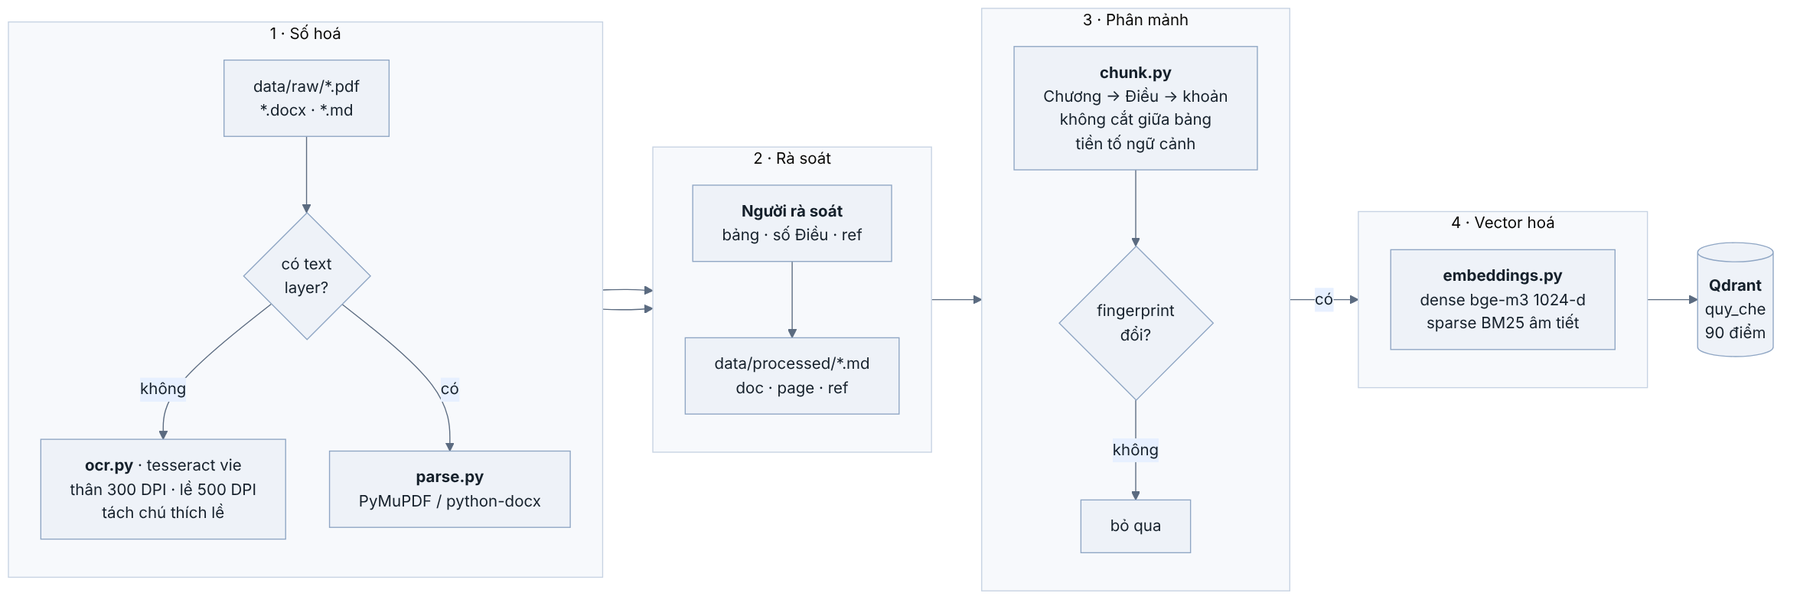
\includegraphics[width=\textwidth]{img/ingest.png}
\caption{Pipeline nạp dữ liệu, từ PDF gốc tới vector trong Qdrant. Bước rà soát của con người
là bắt buộc với bản scan và là ranh giới chất lượng của toàn hệ thống.}
\label{fig:ingest}
\end{figure}

PDF gốc là bản quét, không có lớp văn bản. Hệ thống tự phát hiện điều này (tổng số ký tự trích
được nhỏ hơn 20 ký tự mỗi trang) và chuyển sang OCR bằng Tesseract với gói ngôn ngữ tiếng Việt.
Kết quả OCR được ghi ra Markdown kèm ba loại chú thích máy đọc được:

\begin{codeblock}
<!-- doc: {"doc_id": ..., "number": "285/ĐHBK-ĐT", "effective_year": 2022} -->
<!-- page: 4 -->
<!-- ref: Khoản 3.1, Điều 3, HVu_ĐH | raw: "Khoản 3.1, / Điều 3, / HVu_ĐH" -->
Điều 5. Thời gian đào tạo
5.1 Một số khái niệm thời gian đào tạo
\end{codeblock}

Bản Markdown này sau đó được \textbf{người rà soát bằng mắt}: sửa bảng, kiểm tra số Điều, đối
chiếu chú thích lề. Đây là quyết định thiết kế có chủ ý — OCR tiếng Việt trên bản quét không
bao giờ đạt 100\%, và trong bài toán quy phạm thì một con số sai do OCR sẽ lan thành câu trả
lời sai mà không ai phát hiện. Hệ thống hỗ trợ bằng lệnh kiểm tra cấu trúc, báo các số Điều
thiếu hoặc sai thứ tự và các chú thích lề đọc không rõ.

\begin{notebox}[title={Nguyên tắc}]
Markdown đã rà soát là nguồn chân lý duy nhất. Pipeline không bao giờ ghi đè lên nó: khi PDF
nguồn thay đổi, bản OCR mới được ghi ra file \code{.md.new} để người dùng tự so sánh, chứ không
xoá công sức rà soát đã bỏ ra.
\end{notebox}

\subsection{Giai đoạn 2 — Phân mảnh theo cấu trúc}

Bản Markdown được phân tích thành cây Chương → Điều/Phụ lục → khoản, rồi đóng gói thành chunk
theo quy tắc: \textbf{một Điều là một chunk} nếu vừa ngưỡng token; nếu không vừa thì gom các
khoản liên tiếp cho tới sát ngưỡng; nếu một khoản vẫn quá dài thì cắt giữa các câu, với phần
chồng lấn nhỏ. Chi tiết thuật toán ở mục~\ref{sec:chunk}.

\subsection{Giai đoạn 3 — Vector hoá và lưu trữ}

Mỗi chunk sinh ra hai biểu diễn: vector dense 1024 chiều từ \code{bge-m3}, và vector thưa BM25
tự tính. Cả hai được lưu trong cùng một điểm Qdrant, kèm payload đầy đủ siêu dữ liệu (số Điều,
tiêu đề, danh sách khoản, trang, chú thích nguồn gốc). Việc nạp dữ liệu là \emph{idempotent}:
mã định danh của chunk sinh theo công thức tất định, và một manifest lưu dấu vân tay từng văn
bản, nên chạy lại khi không có gì đổi thì không tốn một lời gọi embedding nào.

\subsection{Giai đoạn 4 — Truy xuất}

\begin{figure}[htbp]
\centering
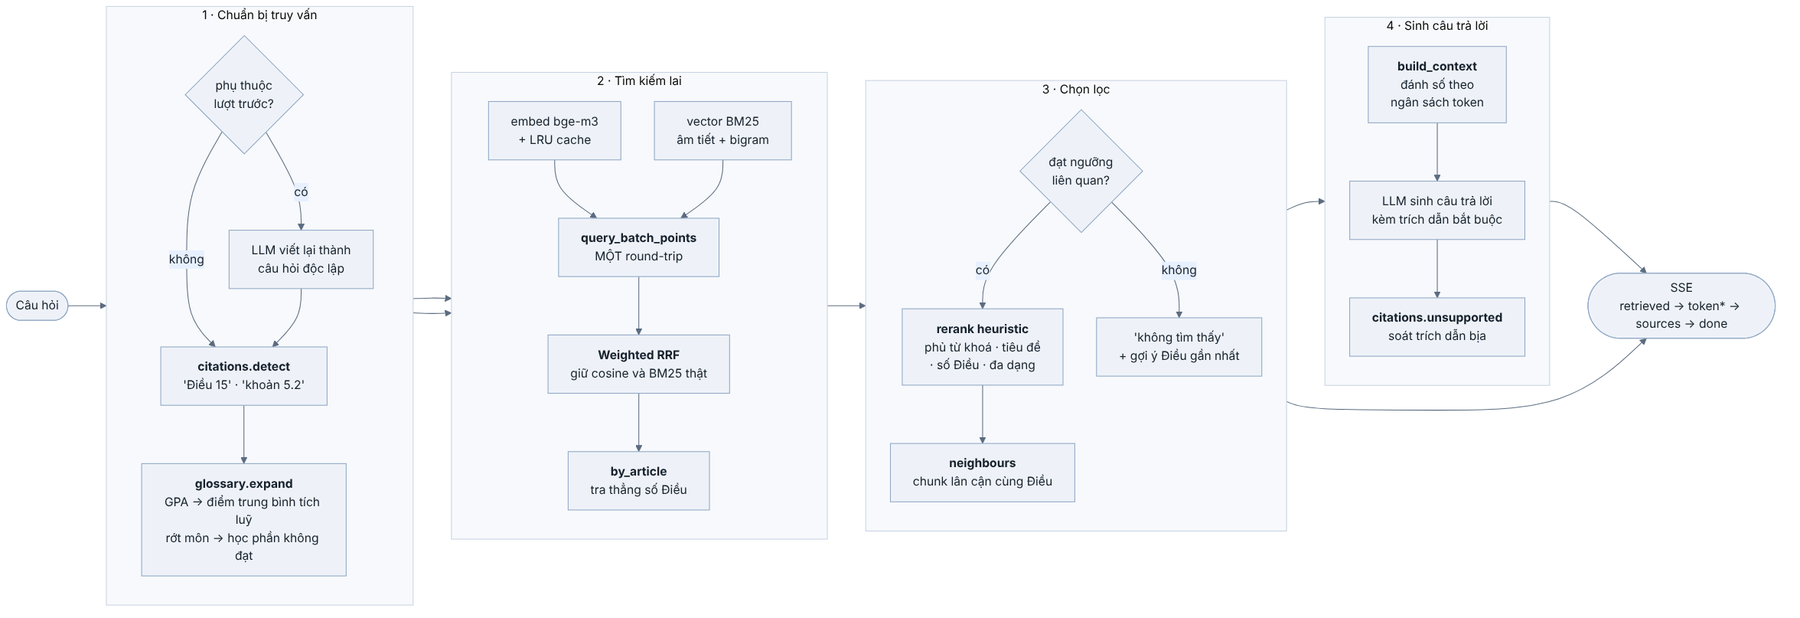
\includegraphics[width=\textwidth]{img/truy-xuat.png}
\caption{Pipeline truy xuất, bốn pha. Toàn bộ pha 1, 3 và phần hợp nhất của pha 2 là tính toán
CPU thuần; mỗi câu hỏi chỉ tốn một lời gọi tới Qdrant và một lời gọi embedding (có bộ nhớ
đệm).}
\label{fig:truyxuat}
\end{figure}

Đây là phần nhận nhiều công sức nhất của đồ án, và là phần quyết định chất lượng. Chi tiết từng
kỹ thuật được trình bày ở chương~\ref{sec:chitiet}.

\subsection{Giai đoạn 5 — Sinh câu trả lời}

Các trích đoạn được đánh số và gắn tiêu đề đầy đủ trước khi đưa vào prompt, nhờ đó mô hình
trích dẫn được tên Điều thật chứ không phải “[1]”. Prompt ràng buộc sáu quy tắc
(mục~\ref{sec:prompt}), và sau khi mô hình viết xong, mọi trích dẫn được đối chiếu ngược lại
với ngữ cảnh.

\subsection{Giai đoạn 6 — Giao diện}

\begin{figure}[htbp]
\centering
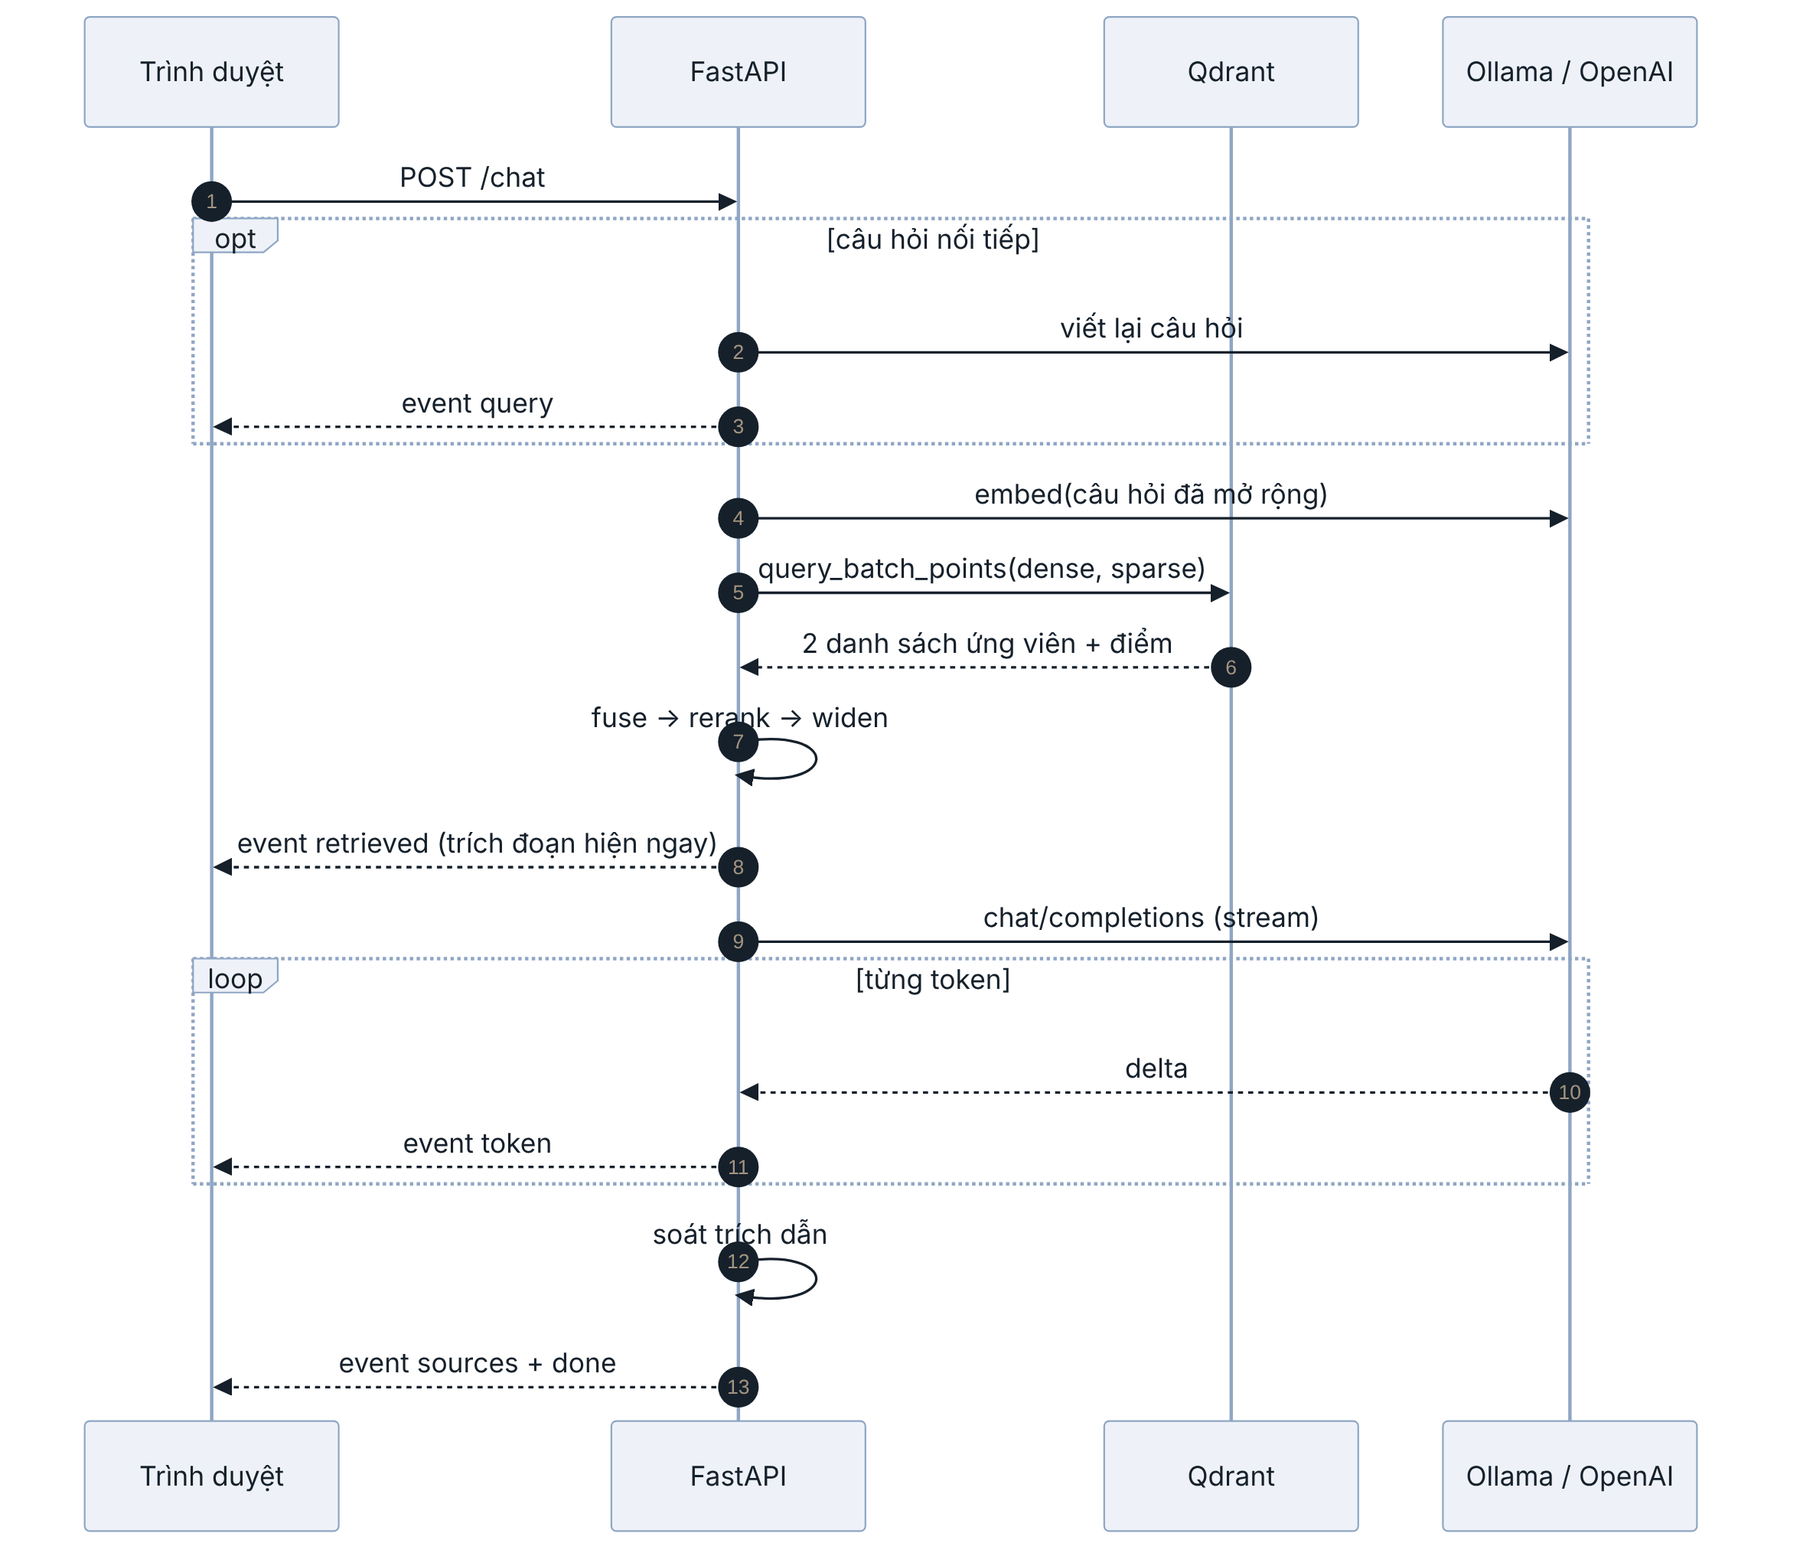
\includegraphics[width=0.78\textwidth]{img/sse.png}
\caption{Trình tự một lượt hỏi đáp. Điểm đáng chú ý là sự kiện \code{retrieved}: trích đoạn tới
trình duyệt trước khi mô hình bắt đầu viết, nên trên máy chỉ có CPU người đọc vẫn có việc để
làm ngay.}
\label{fig:sse}
\end{figure}

\subsection{Giai đoạn 7 — Kiểm thử và đánh giá}

Hai lớp kiểm chứng được xây dựng song song với hệ thống. Lớp thứ nhất là 69 test tự động chạy
trong vài giây, dùng Qdrant in-memory và một embedder băm từ vựng tất định, nên không cần
Ollama, không cần mạng, không cần GPU — điều kiện tiên quyết để bộ test thực sự được chạy
thường xuyên. Lớp thứ hai là bộ 30 câu hỏi vàng đo chất lượng truy xuất trên hệ thống thật.

\chapterbreak
